
%----------------------------------------------------------------------------------------
%	Lecture 1
%----------------------------------------------------------------------------------------

\chapter{Vectors and Dot Product}

\bigbreak
\section{Vectors}

A vector is a quantity that has both a magnitude and a direction.
We usually use a coordinate system to represent vectors.
Usually, we use a cartesian coordinates to represent a vector as its component along the coordinate axis.
We will represent any vector as ${\bf v}$ bold.

$$ {\bf A} = \ijk{a_1}{a_2}{a_3} = \left< a_1, a_2, a_3 \right> $$

We can get the direction by scaling the vector by its length, that is, dividiing it by its length $|{\bf A}|$.
A vector is if it has the same magnitude and direction irrespective of its starting point.
We can find out the length of a vector by the following formula : $$ |{\bf A}| = \sqrt{a_1^2 + a_2^2 + a_3^3} $$

This is true due to the fact that we are using the cartesian coordinates to represent our vector.
So this vector can be seen as the diagonal of a cuboid and using the pythogorean theorem, we can find its length.

\subsection{Scalar Multiplication}
Geometrically, mulitplying a vector by a scalar is the same as rescaling the vector by that scalar.

Numerically, $$ c {\bf A} = c (\ijk{a_1}{a_2}{a_3}) = (\ijk{ca_1}{ca_2}{ca_3}) $$

\subsection{Vector Addition}

Vector addition can be done either geometrically or numerically.
Geometrically, start at any point and then travel in the direction of first vector a distance equal its length.
Then we travel in the direction of the second vector a distance equal to its length.
Finally, the addition of two vectors is the vector from the starting point to the final point.

\begin{figure}[ht!]
	\centering
	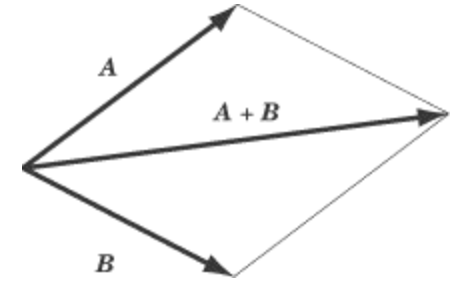
\includegraphics[scale=0.5]{./images/lecture_1_figure_1.png}
	\caption{Geometrycally Adding Vectors}
\end{figure}

In the diagram above, we can see that if both vectors start at the same point then their sum is the diagonal of the parallelogram formed by the two vectors.
Numerically, $$ {\bf A} + {\bf B} = \left< a_1, a_2, a_3 \right> + \left< b_1, b_2, b_3 \right> = \left< a_1 + b_1, a_2 + b_2, a_3 + b_3 \right> $$
or,
$$ {\bf A} + {\bf B} = \ijk{a_1}{a_2}{a_3} + \ijk{b_1}{b_2}{b_3} = \ijk{(a_1 + b_1)}{(a_2 + b_2)}{(a_3 + b_3)} $$


\section{Dot Products}

Definition :
$$
{\bf A} \cdot {\bf B} = \sum a_i b_i = a_1 b_1 + a_2 b_2 + a_3 b_3
$$

Geometrically, let $\theta$ be the angle between vector ${\bf A}$ and ${\bf B}$. Then,
$$ {\bf A} \cdot {\bf B} = |{\bf A}||{\bf B}| \cos \theta $$

What does the geometric definition mean ? And how does it relates to the numerical definition.

First we have, ${\bf A} \cdot {\bf A} = |{\bf A}|^2 \cos(0) = |{\bf A}|^2 = a_1^2 + a_2^2 + a_3^2 $.
So this proves that the geometric definition is the same as the numerical definition when ${\bf A} = {\bf B}$.

Secondly, let ${\bf C} = {\bf B} - {\bf A}$ as you can see in the diagram below.

\begin{figure}[ht!]
	\centering
	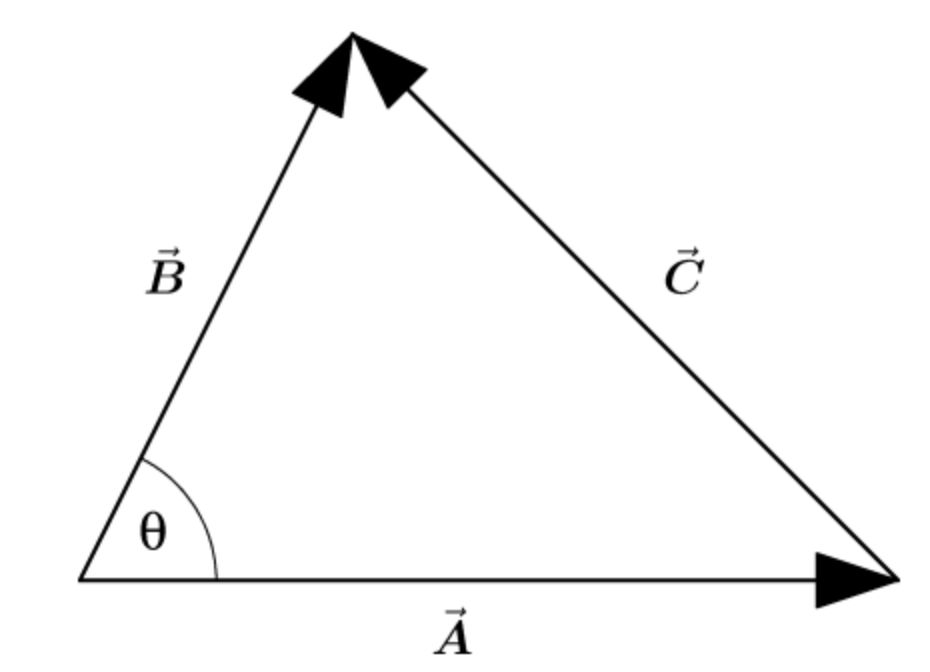
\includegraphics[scale=0.5]{./images/lecture_1_figure_2.png}
	\caption{Law of Cosines \& Dot Product}
\end{figure}

The law of cosines says, $$ |{\bf C}|^2 = |{\bf A}|^2 + |{\bf B}|^2 - 2|{\bf A}||{\bf B}|\cos \theta $$
But we know that, $$|{\bf C}|^2 = {\bf C} \cdot {\bf C} = ({\bf A} - {\bf B}) \cdot ({\bf A} - {\bf B}) $$
The dot product is distributive and commutative. This can be verified from the numerical definition of the dot product.
So,
\begin{eqnarray*}
	|{\bf C}|^2 = {\bf A} \cdot {\bf A} - {\bf A} \cdot {\bf B} - {\bf B} \cdot {\bf A} + {\bf B} \cdot {\bf B} \\
	|{\bf C}|^2 = |{\bf A}|^2 + |{\bf B}|^2 - 2 {\bf A} \cdot {\bf B} \\
	{\bf A} \cdot {\bf B} = |{\bf A}||{\bf B}| \cos \theta
\end{eqnarray*}

Thus, the geometric and numerical definition are equivalent to each other.

\subsection{Uses of Dot Product}

\subsubsection{Finding Angle Between Two Vectors}

The dot product is useful to find out the angles between vectors.
$$ \cos \theta = \frac{ {\bf A} \cdot {\bf B} }{ |{\bf A}| |{\bf B}| } $$

From the above formula, we can also see that the sign of the lengths are always positive.
So, the sign of the dot product is the same as the sign of $\cos \theta$.
$$
\text{Sign of } {\bf A} \cdot {\bf B} :
	\begin{cases}
		> 0 & \quad \text{ if } \theta < 90^{\circ} \\
		= 0 & \quad \text{ if } \theta = 90^{\circ} \\
		< 0 & \quad \text{ if } \theta > 90^{\circ}
	\end{cases}
$$

\subsubsection{Determining Orthoginality}

The second use of the dot product is to figure out orthogonality.
That is, to find whether two vectors are perpendicular to each other or not.

{\bf Example : } Find set of solutions $x + 2y + 3z = 0$.


We can rewrite the equation as $$ (\ijk{1}{2}{3})(\ijk{x}{y}{z}) = 0 $$
Thus, the solutions to this equation is all the points whose vector is perpendicular to $\ijk{1}{2}{3}$.


\subsubsection{Finding Component of {\bf A} along a unit vector $\hat{u}$}

Since the length of a unit vector is $1$, we have,
$$ {\bf A} \cdot \hat{u} = |{\bf A}||\hat{u}| \cos \theta = |{\bf A}|\cos \theta $$